%%%%%%%%%%%%%%%%%%%%%%%%%%%%%%%%%%%%%%%%%%%%%%%%%%%%%%%%%%%%%%%
% Welcome to the MAT320 Homework template on Overleaf -- just edit your
% LaTeX on the left, and we'll compile it for you on the right.
%%%%%%%%%%%%%%%%%%%%%%%%%%%%%%%%%%%%%%%%%%%%%%%%%%%%%%%%%%%%%%%
% --------------------------------------------------------------
% Based on a homework template by Dana Ernst.
% --------------------------------------------------------------
% This is all preamble stuff that you don't have to worry about.
% Head down to where it says "Start here"
% --------------------------------------------------------------

\documentclass[12pt]{article}

\usepackage{graphicx}
\graphicspath{{./images/}}
\usepackage{textcomp} % cent symbol, such as \textcent
\usepackage[margin=1in]{geometry} 
\usepackage{amsmath,amsthm,amssymb}
\usepackage{cancel}
\usepackage{mathtools} % ceiling function
\DeclarePairedDelimiter{\ceil}{\lceil}{\rceil}
% https://tex.stackexchange.com/questions/146306/how-to-make-horizontal-lists
\usepackage[inline]{enumitem} % allows using letters in enumerate list environment

% source: https://stackoverflow.com/questions/3175105/inserting-code-in-this-latex-document-with-indentation

\usepackage{listings}
\usepackage{color}

\definecolor{dkgreen}{rgb}{0,0.6,0}
\definecolor{gray}{rgb}{0.5,0.5,0.5}
\definecolor{mauve}{rgb}{0.58,0,0.82}

\lstset{frame=tb,
	language=C, % language for code listing
	aboveskip=3mm,
	belowskip=3mm,
	showstringspaces=false,
	columns=flexible,
	basicstyle={\small\ttfamily},
	numbers=none,
	numberstyle=\tiny\color{gray},
	keywordstyle=\color{blue},
	commentstyle=\color{dkgreen},
	stringstyle=\color{mauve},
	breaklines=true,
	breakatwhitespace=true,
	tabsize=4
}

\newcommand{\N}{\mathbb{N}}
\newcommand{\Z}{\mathbb{Z}}

\newenvironment{ex}[2][Exercise]{\begin{trivlist}
		\item[\hskip \labelsep {\bfseries #1}\hskip \labelsep {\bfseries #2.}]}{\end{trivlist}}

\newenvironment{sol}[1][Solution]{\begin{trivlist}
		\item[\hskip \labelsep {\bfseries #1:}]}{\end{trivlist}}


\begin{document}

% --------------------------------------------------------------
%                         Start here
% --------------------------------------------------------------

\noindent Sergio Garcia Tapia \hfill

\noindent{\small Computer Systems: A Programmer's Perspective, by Bryant and O'Hallaron} \hfill

\noindent{\small Chapter 5: Optimizing Program Performance}
\noindent\today

\subsection*{Practice Problems}

\begin{ex}{5.1}
	The following problem illustrates the way memory aliasing can cause unexpected program
	behavior. Consider the following procedure to swap to values:
	\begin{lstlisting}
/* Swap value x at xp with value y at yp */
void swap(long *xp, long *yp)
{
	*xp = *xp + *yp;	/* x + y */
	*yp = *xp - *yp;	/* x+y-y = x */
	*xp = *xp - *yp;	/* x+y-x = y */
}
	\end{lstlisting}
	If this procedure is called with \texttt{xp} equal to \texttt{yp}, what effect will it
	have?
\end{ex}

\begin{sol}
	\
	If \texttt{xp} equals \texttt{yp}, meaning that the pointers hold the same memory address,
	then the variables are aliased. As a result, all subsequent assignments set both \texttt{*xp}
	and \texttt{*yp}. The first expression sets \texttt{*xp} (and hence the aliased \texttt{*yp})
	to twice the original value of \texttt{*x}. Then, the next expression evaluates to 0, so \texttt{*yp} and \texttt{*xp} are set 0. The final expression sets \texttt{*xp} (and hence \texttt{*yp}) to \texttt{0 - 0}, or just \texttt{0}.
	
	\
	Therefore, instead of swapping values, both values are set to \texttt{0}.
\end{sol}

\begin{ex}{5.2}
	Later in this chapter we will start with a single function and generate many different
	variants that preserve the function's behavior, but with difference performance
	characteristics. For three of these variants, we found that the run times (in clock
	cycles) can be approximated by the following functions:
	\begin{itemize}
		\item Version 1: $60+35n$
		\item Version 2: $136+4n$
		\item Version 3: $157+1.25n$
	\end{itemize}
	For what values of $n$ would each version be the fastest of the three? Remember
	that $n$ will always be an integer.
\end{ex}

\begin{sol}
	\
	When $n=0$, Version 1 has the smallest value: 60. That is, it requires the least cycles
	per elements. Because it has the greatest slope, it will eventually surpass both
	of the other versions in terms of required cycles per element. Version 1 will intersect Version 2
	when $60+35n=136+4n$, or $31n=76$, making $n$ about $2.45$. Since $n$ is an integer, this
	means we require $n$ to be at least 3. Similarly, Version 1 and Version 3 intersect when
	$60+35n=157+1.25n$. This means $33.75n=97$, so $n$ is about $2.87$, but once again
	$n$ must be an integer so we require it to be 3. At this point, either Version 2 or
	Version 3 is the fastest. These versions intersect when $136+4n=157+1.25n$, so
	$2.75n=21$, meaning $n$ is about $7.6$. Version 2 hs a larger slope, so eventually its
	slope will overcome that of Version 3,; this will happen when $n=8$. However, this means
	that when $n$ is between 3 and 7 (inclusive), Version 2 will have less cycles per element.
	
	\
	Therefore, when $n < 3$, Version 1 is the fastest, followed by Version 2 when 
	$3\leq n < 7$, and lastly, Version 3 is the fastest when $n\geq 8$, requiring 1.25 cycles
	per element.
\end{sol}

\begin{ex}{5.3}
	Consider the following functions:
	\begin{lstlisting}
long min(long x, long y) { return x < y ? x : y; }
long max(long x, long y) { return x < y ? y : x; }
void incr(long *xp, long v) { *xp += v; }
long square(long x) { return x*x; }
	\end{lstlisting}
	The following three code fragments call these functions:
	\begin{enumerate}[label=(\alph*)]
		\item \
		\begin{lstlisting}
for (i = min(x, y); i < max(x, y); incr(&i, 1)
	t += square(i);
		\end{lstlisting}
		\item \
		\begin{lstlisting}
for (i = max(x, y) - 1; i >= min(x, y); incr(&i, -1))
	t += square(i);
		\end{lstlisting}
		\item \
		\begin{lstlisting}
long low = min(x, y);
long high = max(x, y);
for (i = low; i < high; incr(&i, 1))
	t += square(i);
		\end{lstlisting}
	\end{enumerate}
	Assume \texttt{x} equals 10 and \texttt{y} equals 100. Fill int he following
	table indicating the number of times each of the four functions is called
	in code fragments A-C.
	\begin{center}
		\begin{tabular}{ccccc}
			Code & \texttt{min} & \texttt{max} & \texttt{incr} & \texttt{square}\\
			\hline
			A & \makebox[1cm]{\hrulefill} & \makebox[1cm]{\hrulefill} & \makebox[1cm]{\hrulefill} & \makebox[1cm]{\hrulefill}\\
			
			B & \makebox[1cm]{\hrulefill} & \makebox[1cm]{\hrulefill} & \makebox[1cm]{\hrulefill} & \makebox[1cm]{\hrulefill}\\
			
			C & \makebox[1cm]{\hrulefill} & \makebox[1cm]{\hrulefill} & \makebox[1cm]{\hrulefill} & \makebox[1cm]{\hrulefill}\\
		\end{tabular}
	\end{center}
\end{ex}

\begin{sol}
	\
	\begin{center}
		\begin{tabular}{ccccc}
			Code & \texttt{min} & \texttt{max} & \texttt{incr} & \texttt{square}\\
			\hline
			A & 1 & 91 & 90 & 90\\
			
			B & 91 & 1 & 90 & 90\\
			
			C & 1 & 1 & 90 & 90\\
		\end{tabular}
	\end{center}
\end{sol}

\begin{ex}{5.4}
	When we use \texttt{gcc} to compile \texttt{combine3} with command-line option \texttt{-O2},
	we get code with substantially better CPE performance than with \texttt{-O1}:
	\begin{center}
		\begin{tabular}{ccccccc}
			{} & {} & {} & \multicolumn{2}{c}{Integer} & \multicolumn{2}{c}{Floating point}\\
			Function & Page & Method & \texttt{+} & \texttt{*} & \texttt{+} & \texttt{*}\\
			\hline
			\texttt{combine3} & 513 & Compiled \texttt{-O1} & 7.17 & 9.02 & 9.02 & 11.03\\
			\texttt{combine3} & 513 & Compiled \texttt{-O2} & 1.60 & 3.01 & 3.01 & 5.01\\
			\texttt{combine4} & 513 & Accumulate in temporary & 1.27 & 3.01 & 3.01 & 5.01\\
		\end{tabular}
	\end{center}
	We achieve performance comparable to that of \texttt{combine4}, except for the case of
	integer sum, but even it improves significantly. On examining the assembly code generated
	by the compiler, we find an interesting variant of the inner loop:
	\begin{lstlisting}[language={}]
# Inner loop of combine3, data_t = double, OP = *. Compiled -O2
# dest in %rbx, data+i in %rdx, data+length in %rax
# Accumulated product in %xmm0
.L22:								# loop:
	vmulsd	(%rdx), %xmm0, %xmm0	#	Multiply product by data[i]
	addq	$8, %rdx				# 	Increment data + i
	cmpq	%rax, %rdx				#	Compare to data+length
	vmovsd	%xmm0, (%rbx)			# 	Store product at dest
	jne		.L22					#	If !=, goto loop
	\end{lstlisting}
	We can compare this to the version created with optimization level 1:
		\begin{lstlisting}[language={}]
# Inner loop of combine3, data_t = double, OP = *. Compiled -O1
# dest in %rbx, data+i in %rdx, data+length in %rax
.L17:								# loop:
	vmovsd	(%rbx), %xmm0			#	Read product from dest
	vmulsd	(%rdx), %xmm0, %xmm0	#	Multiply product by data[i]
	vmovsd	%xmm0, (%rbx)			#	Store product at dest
	addq	$8, %rdx				# 	Increment data + i
	cmpq	%rax, %rdx				#	Compare to data+length
	jne		.L22					#	If !=, goto loop
	\end{lstlisting}
	We see that, besides some reordering of instructions, the only difference is that the
	more optimized version does not contain the \texttt{vmovsd} implementing the read from
	the location designated by \texttt{dest} (line 2).
	\begin{enumerate}[label=(\alph*)]
		\item How does the role of register \texttt{\%xmm0} differ in these two loops?
		\item Will the more optimized version faithfully implement the C code of \texttt{combine3},
		including when there is memory aliasing between \texttt{dest} and the vector
		\texttt{data}?
		\item Either explain why this optimization preserves the desired behavior, or give an
		example where it would produce different results than the less optimized code.
	\end{enumerate}
\end{ex}

\begin{sol}
	\
	\begin{enumerate}[label=(\alph*)]
		\item In the version of \texttt{compare3} compiled with \texttt{-O2}, the \texttt{\%xmm0}
		register holds the value accumulated so far. Since this value is used in the next iteration,
		there is no need to read memory to obtain it; it can be directly used from \texttt{\%xmm0}.
		This is in contrast with with the version of \texttt{compare3} compiled with \texttt{-O1},
		where rather than reading the accumulated value from \texttt{\%xmm0}, it is read from
		memory before operating on it.
		\item Yes, the more optimized version faithfully implements \texttt{combine3}.
		In both cases, the computed value is written to the destination every iteration.
		Therefore, the value read from the accumulated register \texttt{\%xmm0} in the version
		compiled with \texttt{-O2} will always match the value read via the memory reference
		\texttt{(\%rbx)} in version compiled with \texttt{-O1}.
		\item The optimized version preserves the desired behavior by updating the destination
		with the current value in \texttt{dest} in every iteration, rather than doing so
		once at the end after the loop ends.
	\end{enumerate}
\end{sol}

\begin{ex}{5.5}
	Suppose we wish to write a function to evaluate a polynomial, where a polynomial of degree
	$n$ is defined to have a set of coefficients $a_0,a_1,\ldots,a_n$. For a value $x$, we
	evaluate the polynomial by computing
	\[
	a_0+a_1x+a_2x^2+\cdots+a_nx^n
	\]
	This evaluation can be implemented by the following function, having as arguments an array
	of coefficients \texttt{a}, a value \texttt{x}, and the polynomial of degree \texttt{degree}
	(the value $n$ in the polynomial expression above). In this function, we compute both the
	successive terms of the equation and the successive powers of $x$ within a single loop:
	\begin{lstlisting}
double poly(double a[], double x, long degree)
{
	long i;
	double result = a[0];
	double xpwr = x;	/* Equals x^i at start of loop */
	for (i = 1; i <= degree; i++) {
		result += a[i] * xpwr;	/* Line 7 */
		xpwr = x * xpwr;		/* Line 8 */
	}
	return result;
}
	\end{lstlisting}
	\begin{enumerate}[label=(\alph*)]
		\item For degree $n$, how many additions and how many multiplications does this code
		perform?
		\item On our reference machine, with arithmetic operations having the latencies shown in
		Figure 5.12, we measure the CPE for this function to be 5.00. Explain how this CPE arises
		based on the data dependencies due to the operations implementing lines 7-8 of the
		function.
	\end{enumerate}
\end{ex}

\begin{sol}
	\
	\begin{enumerate}[label=(\alph*)]
		\item There are $n$ additions due to the statement \texttt{i++}, and $n$ additions
		due to the \texttt{result +=} statement, for a total of $2n$ additions. There
		are $2n$ multiplications, where $n$ come from the first statement in the loop
		which multiplies a coefficient by a power of $x$, and $n$ from the second coming
		from computing the next power of $x$.
		\item On line 7, we see that \texttt{result} is used as both a source and destination,
		making its associated floating point register a \emph{loop} register. The \texttt{a[i]}
		and \texttt{x} expressions are associated with a \emph{read-only} register, since they are
		only used as source values and not updated Finally, the \texttt{xpwr} expression is used as
		a source and destination value, making its associated register at \texttt{loop} register.
		See Figure~\ref{fig:ex-05-05}.
		\begin{figure}
			\centering
			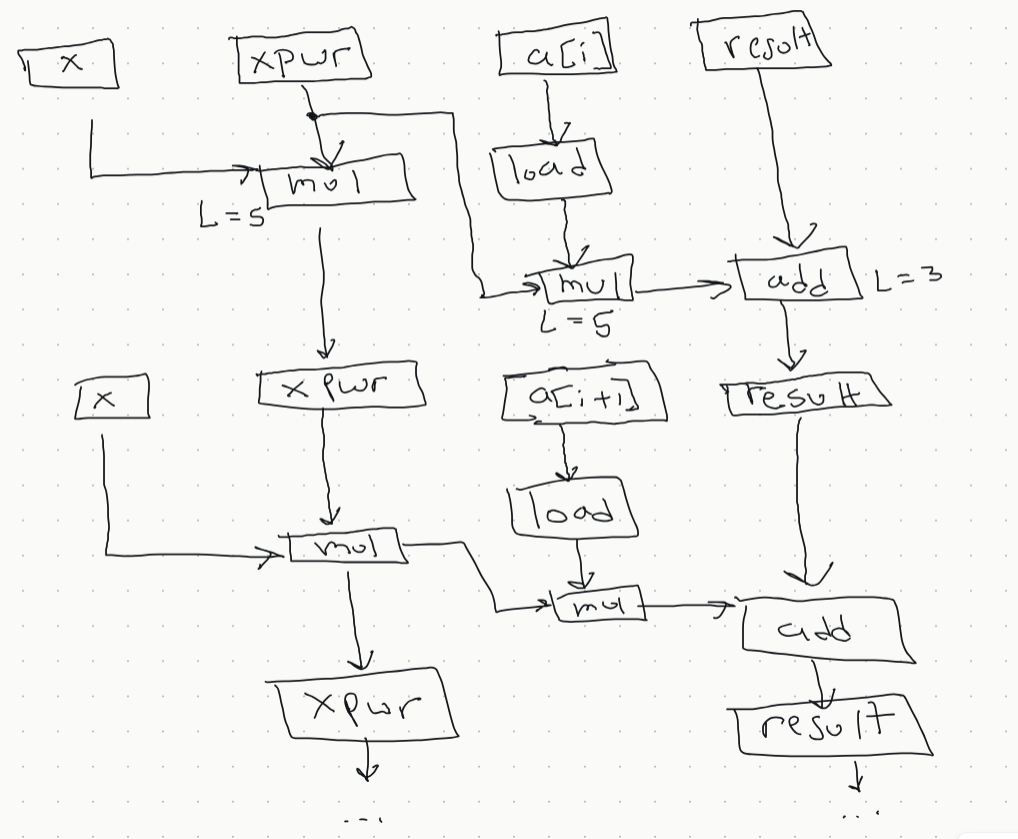
\includegraphics[width=0.6\textwidth]{exercise-05-05.png}
			\caption{Exercise 05-05: Data flow graph representing dependencies during $i$-th
				iteration}
			\label{fig:ex-05-05}
		\end{figure}
		
		\
		At first, it may seem like the latency is 8 cycles because the addition on
		line 7 cannot start until the product \texttt{a[i] * xpwr} is computed. Let
		the moment before the first iteration correspond to cycle 0. Since the capacity of
		the floating point multiplication is 2 and the latency is 5, and the two products
		in each iteration are independent, the two products \texttt{a[0] * pwr} and
		\texttt{x * xpwr} occur simultaneously.
		
		\
		On cycle 5, the product \texttt{a[0] * xpwr} has completed, so the addition portion
		of \texttt{result += a[0] * xpwr} may begin. Similarly, the floating-point multiplication
		operations \texttt{a[1] * xpwr} and \texttt{x * xpwr} can begin also. Since the latency of
		floating point addition is 3 cycles, the addition \texttt{result += a[0] * xpwr} finishes 
		by cycle 8. However, the multiplications are still happening. As a result, the addition in
		\texttt{result += a[1] * xpwr} cannot begin. By cycle 10, the two multiplications
		from the second iteration have ended, and at this point the addition
		\texttt{result += a[1] * xpwr} can take place, ending at cycle 13.
		
		\
		Altogether, the \texttt{xpwr} variable updates every 5 cycles, while the \texttt{result}
		variable also updates every 5 cycles. The difference is that \texttt{result} lags 3
		cycles behind. For example, the \texttt{xpwr} variable is updated at cycles 5, 10, 15,
		and so on. Meanwhile, the \texttt{result} variable is updated at cycles 8, 13, 18, and
		so on, After $n$ iterations, the last value of \texttt{xpwr} will have computed after
		$5n$ cycles, whereas the last value of \texttt{result} will be computed after $5n+3$
		cycles. 
		
	\end{enumerate}
\end{sol}

\begin{ex}{5.6}
	Let us continue exploring ways to evaluate polynomials as described in Practice Problem 5.5.
	We can reduce the number of multiplications in evaluating a polynomial by applying
	\emph{Horner's Method}, named after British mathematician William G. Horner (1787-1837).
	The idea is to repeatedly factor out powers of $x$ to get the following evaluation:
	\[
	a_0+x(a_1+x(a_2+\cdots+x(a_{n-1}+xa_n)\cdots))
	\]
	Using Horner's method, we can implement polynomial evaluation using the following code:
	\begin{lstlisting}
/* Apply Horner's method */
double polyh(double a[], double x, long degree)
{
	long t;
	double result = a[degree];
	for (i = degree-1; i>=0 ; i--)
		result = a[i] + x * result;	/* Line 7 */
	return result;
}
	\end{lstlisting}
	\begin{enumerate}[label=(\alph*)]
		\item For degree $n$, how many additions and how many multiplications does this code
		perform?
		\item On our reference machine, with the arithmetic operations having the latencies
		shown in Figure 5.12, we measure the CPE for this function to be 8.00. Explain how
		this CPE arises based on the data dependencies formed between iterations due to the
		operations implementing line 7 of this function.
		\item Explain how the function shown in Practice Problem 5.5 can run faster, even though
		it requires more operations.
	\end{enumerate}
\end{ex}

\begin{sol}
	\
	\begin{enumerate}[label=(\alph*)]
		\item Considering \texttt{i--} to be an addition of \texttt{-1}, there are
		$n$ additions attributed to it, and $n$ additions attributed to the loop
		statement. There are $n$ multiplications inside the loop. Therefore, there's
		a total of $2n$ additions and $n$ multiplications.
		\item Figure~\ref{fig:ex-05.06} shows the data graph representing the dependencies
		in the $i$-th iteration. The \texttt{result} variable goes through two operations
		in series; multiplication by \texttt{x} and then it is added to \texttt{a[i]}.
		The multiplication takes 5 cycles while the addition takes 3 cycles (on the
		reference machine), so the latency is at least 8 cycles, consistent with the
		CPE.
		\begin{figure}
			\centering
			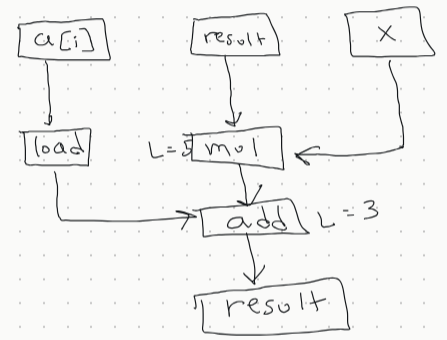
\includegraphics[width=0.5\textwidth]{exercise-05-06.png}
			\caption{Exercise 05-06: Data-flow graph representing dependencies during
				$i$-th iteration}
			\label{fig:ex-05.06}
		\end{figure}
		\item The critical path in Practice Problem 5.5 involves only multiplication, which takes
		5 cycles. Because the capacity is 2, both floating-point multiplications occur
		simultaneously, taking up 5 cycles. The addition depends on the result of the
		first of these two products, and thus it can occur every 5 cycles. The critical
		path is therefore the chain of \texttt{xpwr} computations.
		
		\
		In contrast, Horner's method introduces a data dependency, whereby as indicated
		by Figure~\ref{fig:ex-05.06}. Now both multiplication and addition are on the
		critical path of \texttt{result}, leading to the higher CPE.
	\end{enumerate}
\end{sol}

\begin{ex}{5.7}
	Modify the code for \texttt{combine5} to unroll the loop by a factor of $k=5$.
\end{ex}

\begin{sol}
	\
	For $5\times 1$ loop unrolling, we increment the iteration index by $5$ each time.
	Also, we operate on $5$ operands. To ensure we do not overrun the array bounds, we
	set the limit to $length - 5 + 1$: 
	\begin{lstlisting}
/* 5 x 1 loop unrolling */
void combine5(vec_ptr, data_t *dst)
{
	long i;
	long length = vec_length(v);
	long limit = length - 5 + 1;
	data_t *data = get_vec_start(v);
	data_t acc = IDENT;
	
	/* Combine 2 elements at a time */
	for (i = 0; i < limit; i += 5) {
		acc = ((((acc OP data[i])
								OP data[i+1])
								OP data[i+2])
								OP data[i+3]) 
								OP data[i+4];
	}

	/* Finish any remaining elements */
	for (; i < length; i++) {
		acc = acc OP data[i];
	}
	*dest = acc;
}
	\end{lstlisting}
\end{sol}

\begin{ex}{5.8}
	Consider the following function for computing the product of an array of $n$ double-precision
	numbers. We have unrolled the loop by a factor of $3$.
	\begin{lstlisting}
double aprod(double a[], long n)
{
	long i;
	double x, y, z;
	double r = 1;
	for (i = 0; i < n-2; i += 3) {
		x = a[i]; y = a[i+1]; z = a[i+2];
		r = r * x * y * z;	/* Product computation */
	}
	for (; i < n; i++)
		r *= a[i];
	return r;
}
	\end{lstlisting}
	For the line labeled ``\texttt{Product computation}," we can use parentheses to create five
	different associations of the computation as follows:
	\begin{lstlisting}
r = ((r * x) * y) * z;	/* A1 */
r = (r * (x * y)) * z;	/* A2 */
r = r * ((x * y) * z);	/* A3 */
r = r * (x * (y * z));	/* A4 */
r = (r * x) * (y * z);	/* A5 */
	\end{lstlisting}
	Assume we run these functions on a machine where floating-point multiplication has a
	latency of 5 clock cycles. Determine the lower bound on the CPE set by the data
	dependencies of the multiplication. (\texttt{Hint}: It helps to draw a data-flow
	representation of how \texttt{r} is computed on every iteration.)
\end{ex}

\begin{sol}
	\
	For \texttt{A1}, see the data flow diagram in Figure~\ref{fig:ex-05-08-a1}. There are
	3 multiplications for each iteration on the critical path, and around $n/3$ iterations,
	so overall there are $n$ multiplications in the critical path. Since the latency of
	floating-point multiplication is 5 clock cycles, this leads to a CPE of around 5.0.
	\begin{figure}
		\centering
		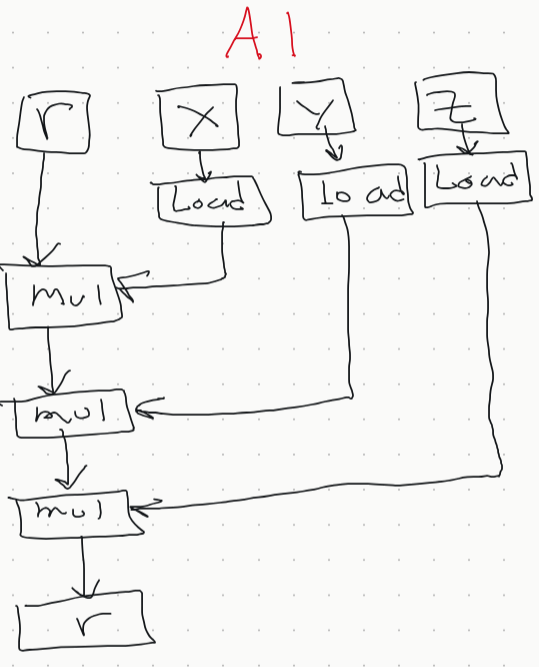
\includegraphics[width=0.4\textwidth]{exercise-05-08-a1.png}
		\caption{Exercise 05-08: Association A1}
		\label{fig:ex-05-08-a1}
	\end{figure}
	
	\
	For \texttt{A2}, see the data flow diagram in Figure~\ref{fig:ex-05-08-a2}. The first
	multiplication on the critical path to compute \texttt{r} cannot start until the
	product \texttt{x * y} has been computed. The effect of this is that there is a lag
	of 5 clock cycles, but ultimately, there are 2 multiplications on the critical path
	of for each iteration. With around $n/3$ iterations, this means there are around
	$2n/3$ multiplications altogether. Since each multiplication has a latency of 5 clock
	cycles, this leads to a CPE of around $5\cdot \frac{2}{3}\approx 3.33$.
	\begin{figure}
		\centering
		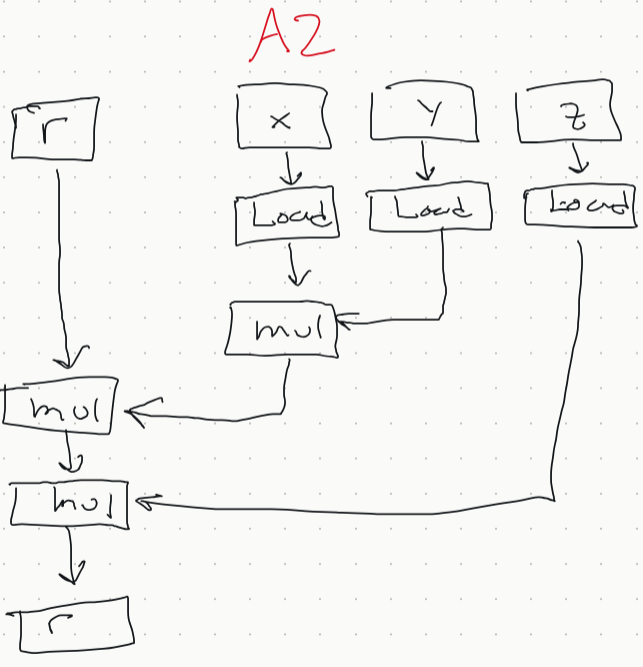
\includegraphics[width=0.4\textwidth]{exercise-05-08-a2.png}
		\caption{Exercise 05-08: Association A2}
		\label{fig:ex-05-08-a2}
	\end{figure}

	\
	For \texttt{A3}, see the data flow diagram in Figure~\ref{fig:ex-05-08-a3}. In cycle 0,
	the product \texttt{x * y}, which is \texttt{a[0] * a[1]} is computed, while the other ones
	are put on hold since the depend on this result. In cycle 5, the product \texttt{(x * y) * z}
	is computed with the result of \texttt{x * y} that has already been computed, but the
	product involving \texttt{r} is still on hold to wait for this result. However, the
	product \texttt{x * y} or equivalently \texttt{a[3] * a[4]} in the next iteration starts
	in cycle 5 as well. In cycle 10, \texttt{r} begins to compute, and \texttt{(x * y) * z}
	also begins to compute for the next iteration, because \texttt{x * y} has already been
	computed. Moreover, \texttt{a[6] * a[7]} from the next iteration also begins in cycle 10. In cycle 15, \texttt{(a[3] * a[4]) * a[5]} from the previous iteration has already computed, so
	the next value of \texttt{r} can compute, while \texttt{(a[6] * a[7]) * a[8]} and
	and \texttt{a[10] * a[11]} compute. In cycle 20, the next value of \texttt{r} can compute
	as \texttt{r * ((a[6] * a[7]) * a[8])}, while \texttt{(a[10] * a[11]) * a[12]} and
	\texttt{a[13] + a[14]} compute. Altogether, \texttt{r} begins to compute every 5 cycles, 
	lagging behind the other products. Since there are $n/3$ iterations, this implies
	a CPE of around $5\cdot (1/3)\approx 1.67$.
	\begin{figure}
		\centering
		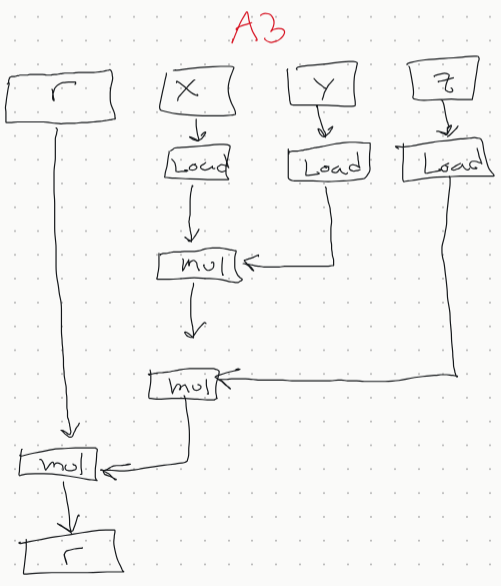
\includegraphics[width=0.4\textwidth]{exercise-05-08-a3.png}
		\caption{Exercise 05-08: Association A3}
		\label{fig:ex-05-08-a3}
	\end{figure}
	
	\
	For \texttt{A4}, see the data flow diagram in Figure~\ref{fig:ex-05-08-a4}. The
	CPE is around 5.0 just like in \texttt{A3}.
	\begin{figure}
		\centering
		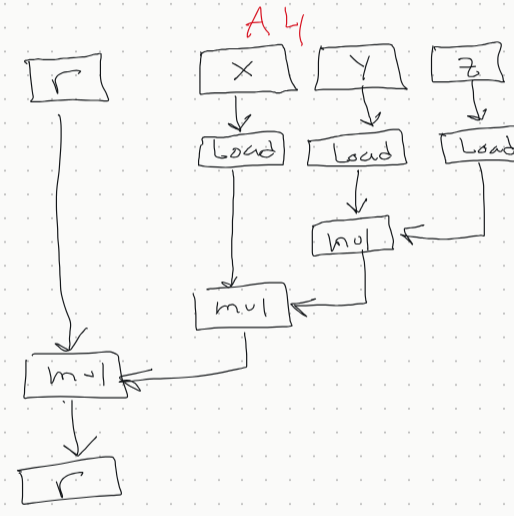
\includegraphics[width=0.4\textwidth]{exercise-05-08-a4.png}
		\caption{Exercise 05-08: Association A4}
		\label{fig:ex-05-08-a4}
	\end{figure}

	\
	For \texttt{A5}, see the data flow diagram in Figure~\ref{fig:ex-05-08-a5}. This
	version has 2 multiplications on the critical path, so it has a CPE of around $3.33$
	just like in \texttt{A2}.
	\begin{figure}
		\centering
		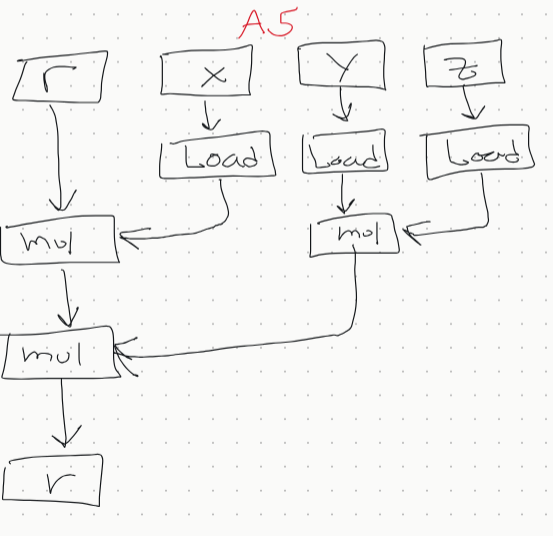
\includegraphics[width=0.4\textwidth]{exercise-05-08-a5.png}
		\caption{Exercise 05-08: Association A5}`
		\label{fig:ex-05-08-a5}
	\end{figure}
\end{sol}
\begin{ex}{5.9}
	The traditional implementation of the merge step of mergesort requires three loops:
	\begin{lstlisting}
void merge(long src1[], long src2[], long dest[], long n) {
	long i1 = 0;
	long i2 = 0;
	long id = 0;
	while (i1 < n && i2 < n) {
		if (src1[i1] < src2[i2])	/* line 6 */
			dest[id++] = src1[i1++];
		else
			dest[id++] = src1[i2++];
	}
	while (i1 < n)
		dest[id++] = src1[i1++];
	while (i2 < n)
		dest[id++] = src2[i2++];
}
	\end{lstlisting}
	The branches caused by comparing variables \texttt{i1} and \texttt{i2} to \texttt{n} have
	good prediction performance --- the only mispredictions occurs when they first become false.
	The comparison between values \texttt{src1[i1]} and \texttt{src2[i2]} (line 6), on the other
	hand, is highly unpredictable for typical data. This comparison controls a conditional
	branch, yielding a CPE (where the number of elements is $2n$) of around 15.0 when run on
	random data.
	
	\
	Rewrite the code so that the effect of the conditional statement in the first loop (lines 6--9)
	can be implemented with a conditional move.
\end{ex}

\begin{sol}
	\
	The book mentions that a functional style, where conditional operations are used to compute
	values and then update program state with these values, are more amenable to translation
	into conditional data transfers than an imperative style, where conditionals are used to
	selectively update program state. This means we need to eliminate the \texttt{if-else} statement.
	
	The solution provided by the authors, presented below, makes use of the fact that the result of
	the assignment and index updates
	depend on the result of \texttt{a < b}. In C, the result is 1 when the comparison is true,
	so the 1 can be used to increase \texttt{i1}; similarly, \texttt{1 - aLTb} will be 0
	in this case, which can be used to update \texttt{i2}. Hence, \texttt{aLTb} is used to
	assign the correct value to \texttt{dest} and the values of \texttt{i1}, \texttt{i2}, and
	\texttt{id} are computed concurrently. Together with the fact that \texttt{a} and \texttt{b}
	are fetched concurrently, the code becomes amenable to implementation with a conditional move.
	\begin{lstlisting}
void merge(long src1[], long src2[], long dest[], long n) {
	long i1 = 0;
	long i2 = 0;
	long id = 0;
	while (i1 < n && i2 < n) {
		long a = src1[i1];
		long b = src2[i2];
		int aLTb = a < b;
		dest[id++] = aLTb ? a : b;
		i1 += aLTb;
		i2 += (1-aLTb);
	}
	while (i1 < n)
		dest[id++] = src1[i1++];
	while (i2 < n)
		dest[id++] = src2[i2++];
}
	\end{lstlisting}
\end{sol}

\begin{ex}{5.10}
	As another example of code with potential load-store interactions, consider the following
	function to copy the contents of one array to another:
	\begin{lstlisting}
void copy_array(long *src, long *dest, long n)
{
	long i;
	for (i = 0; i < n; i++)
		dest[i] = src[i];
}
	\end{lstlisting}
	Suppose \texttt{a} is an array of length $1000$ initialized so that each element of
	\texttt{a[i]} equals $i$.
	\begin{enumerate}[label=(\alph*)]
		\item What would be the effect of calling \texttt{copy\_array(a+1, a, 999)}?
		\item What would be the effect of calling \texttt{copy\_array(a, a+1, 999)}?
		\item Our performance measurements indicate that the call of part A has a CPE of 1.2
		(which drops to 1.0 when the loop is unrolled by a factor of 4), while the call of part
		B has a CPE of 5.0. To what factor do you attribute this performance difference?
		\item What performance would you expect for the call \texttt{copy\_array(a, a, 999)}
	\end{enumerate}
\end{ex}

\begin{sol}
	\
	\begin{enumerate}[label=(\alph*)]
		\item Initially, the array has values 0 through 999, inclusive. Afterwards, it will
		have values 1 through 999 at positions 0 through 998, respectively. The value at position
		999, namely \texttt{a[999]}, will remain unchanged, with a value of 999.
		\item The computation sets all elements to the value of \texttt{a[0]}, which is 0.
		\item In part A, the load operation and store operation refer to distinct addresses,
		so they can compute independently. In part B, the load operation depends on the pending
		store operation from the previous iteration, introducing a data dependency that becomes
		the critical path. Since the reference machine has a 4 cycle access time, this must
		complete before it can be accessed for the next iteration, leading to the 5.0 CPE.
		\item I would expect a CPE of 1.0 because even though the store and read address
		are the same, there is no pending store. In other words, there is no pending right
		when the address is initially computed; the write happens afterwards. Therefore,
		there is no dependency that would lead to the 4.0 CPE penalty described above.
	\end{enumerate}
\end{sol}

\begin{ex}{5.11}
	We saw that our measurements of the prefix-sum function \texttt{psum1} (Figure 5.1) yield
	a CPE of 9.00 on a machine where the basic operation to be performed, floating-point addition,
	has a latency of just 3 clock cycles. Let us try to understand why our function performs so
	poorly.
	
	\
	The following is the assembly code for the inner loop of the function:
	\begin{lstlisting}[language={}]
Inner loop of psum1
a in %rdi, i in %rax, cnt in %rdx
.L5:										# loop:
	vmovss	-4(%rsi,%rax,4), %xmm0			# 	Get p[i-1]
	vaddss	(%rdi,%rax,4), %xmm0, %xmm0		# 	Add a[i]
	vmovss	%xmm0, (%rsi,%rax,4)			#	Store at p[i]
	addq	$1, %rax						#	Increment i
	cmpq	%rdx, %rax						#	Compare i:cnt
	jne		.L5								#	If !=, goto loop
	\end{lstlisting}
	Perform an analysis similar to those shown for \texttt{combine4} (Figure 5.14) and for
	\texttt{write\_read} (Figure 5.36) to diagram the data dependencies created by this loop,
	and hence the critical path that forms as the computation proceeds. Explain why the CPE is
	so high.
\end{ex}

\begin{sol}
	\
	The following is the code for \texttt{psum1}:
	\begin{lstlisting}
/* Compute prefix sum of vector a */
void psum1(float a[], float p[], long n)
{
	long i;
	p[0] = a[0];
	for (i= 1; i < n; i++)
		p[i] = p[i-1] + a[i];
}
	\end{lstlisting}
	There is a data dependency due to the fact that \texttt{p[i]} is written to in the $i$-th
	iteration, and read from in the $(i+1)$-th iteration. Only then can the floating-point
	addition with \texttt{a[i]} take place. Therefore the critical path contains the
	store operation, the load operation, and the floating-point addition. The floating-point
	addition incurs 3 clock cycles on the CPE. The dependency between the store and load
	operations incurs a penalty of about 6 clock cycles on the CPE, explaining the 9.0
	CPE.
\end{sol}

\begin{ex}{5.12}
	Rewrite the code for \texttt{psum1} (Figure 5.1) so that it does not need to
	repeatedly retrieve the value of \texttt{p[i]} from memory. You do not need to use
	loop unrolling. We measured the resulting code to have a CPE Of 3.00, limited by the
	latency of the floating-point addition.
\end{ex}

\begin{sol}
	\
	To eliminate the dependency, I have introduced an accumulator variable \texttt{acc},
	playing the role of \texttt{p[i-1]} in the original implementation. Its value is computed
	by adding \texttt{a[i]}, giving the new value of \texttt{p[i]}. This will be considered
	the old value in the next iteration, which instead of being read from \texttt{p[i-1]}
	will already be present in \texttt{acc}.
	\begin{lstlisting}
/* Compute prefix sum of vector a */
void psum1_improved(float a[], float p[], long n) {
	long i;
	float acc = a[0];
	p[0] = acc;
	for (i=1; i < n; i++) {
		acc += a[i];
		p[i] = acc;
	}
}
	\end{lstlisting}
\end{sol}

\begin{ex}{5.13}
	Suppose we wish to write a procedure that computes the inner product of two vectors
	\texttt{u} and \texttt{v}, An abstract version of the function has a CPE of $14$--$18$
	with x86-64 for different types of integer and floating-point data. By doing the same
	sort of transformations we did to transform the abstract program \texttt{combine1} into
	the more efficient \texttt{combine4}, we get the following code:
	\begin{lstlisting}
/* Inner product. Accumulate in temporary */
void inner4(vec_ptr u, vec_ptr v, data_t *dest)
{
	long i;
	long length = vec_length(u);
	data_t *udata = get_vec_start(u);
	data_t *vdata = get_vec_start(v);
	data_t sum = (data_t) 0;
	
	for (i = 0; i < length; i++) {
		sum = sum + udata[i] * vdata[i];
	}
	*dest = sum;
}
	\end{lstlisting}
	Our measurements show that this function has CPEs of 1.50 for integer data and 3.00 for
	floating-point data. For data type \texttt{double}, the x86-64 assembly code for the
	inner loop is as follows:
	\begin{lstlisting}[language=={}]
# Inner loop of inner4, data_t = double, OP = *
udata in %rbp, vdata in %rax, sum in %xmm0
.L15:										loop:
	xmovsd	0(%rbp,%rcx,8), %xmm1				Get udata[i]
	vmulsd	(%rax,%rcx,8), %xmm1, %xmm1			Multiply by vdata[i]
	vaddsd	%xmm1, %xmm0, %xmm0					Add to sum
	addq	$1, %rcx							Increment i
	cmpq	%rbx, %rcx							Compare i:limit
	jne		.L15								If !=, goto loop
	\end{lstlisting}
	Assume that the function units have the characteristics listed in Figure 5.12. Namely:
	\begin{center}
		\begin{tabular}{c|ccc|ccc}
			{} & \multicolumn{3}{c}{Integer} & \multicolumn{3}{c}{Floating point}\\
			\hline
			Operaton & Latency & Issue & Capacity & Latency & Issue & Capacity\\
			\hline
			Addition & 1 & 1 & 4 & 3 & 1 & 1\\
			Multiplication & 3 & 1 & 1 & 5 & 1 & 2\\
			Division & 3--30 & 3--30 & 1 & 3--15 & 3--15 & 1
		\end{tabular}
	\end{center}
	\begin{enumerate}[label=(\alph*)]
		\item Diagram how this instruction sequence would be decoded into operations and show
		how the data dependencies between them would create a critical path of operations, in the
		style of Figures 5.13 and 5.14.
		\item For data type \texttt{double}, what lower bound on the CPE is determined by the
		critical path?
		\item Assuming similar instruction sequences for the integer code as well, what lower
		bound on the CPE is determined by the critical path for integer data?
		\item Explain how the floating-point versions can have CPEs of 3.00, even though
		the multiplication operation requires 5 clock cycles.
	\end{enumerate}
\end{ex}

\begin{sol}
	\
	\begin{enumerate}[label=(\alph*)]
		\item See Figure~\ref{fig:ex-05.13a}.
		\begin{figure}
			\centering
			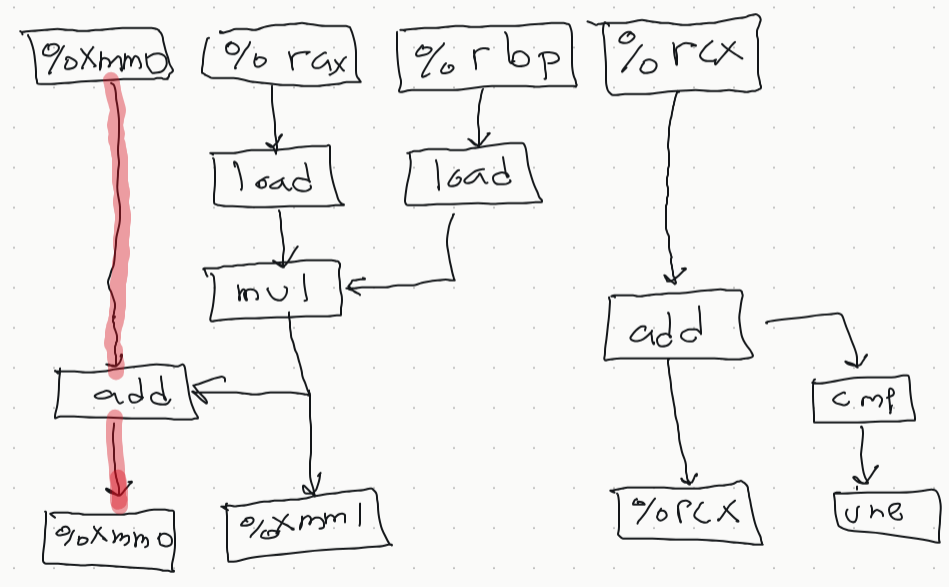
\includegraphics[width=0.6\textwidth]{exercise-05-13a}
			\caption{Exercise 5-13a: Data-dependency flow diagram}
			\label{fig:ex-05.13a}
		\end{figure}
		\item The critical involves the operations updating \texttt{\%xmm0}, the register
		of the accumulation variable \texttt{sum}, via the \texttt{add} operation. The
		multiplication is not involved in a data-dependency chain with loop registers,
		so it can be pipelined. That means that although any one multiplzugh the multiplication
		for the first iteration has not completed on cycle 1, the multiplication for the
		second iteration can still begin on that cycle. Therefore, at cycle 3, the multiplication
		for the first iteration is available, at cycle 4 the multiplication for the second
		iteration is available, and so on.
		
		\
		Since the loop register \texttt{\%xmm0} depends on the floating point addition,
		the fact that it has a latency of 3 on the reference machine determines a
		lower bound of 3.0 for the CPE.
		\item A similar argument applies as before, so both loop registers \texttt{\%rcx}
		and the register holding \texttt{\%sum} constitute critical paths. Since addition
		has a latency of 1, the lower bound for the CPE is 1.0 for integer data. The
		implementation's CPE is 1.50, meaning that the bottleneck is elsewhere, such
		as the overhead of comparison operations and loads.
		\item As explained in part (b), pipelining and the fact that the multiplication is not
		in the critical path implies that the results of the multiplications will
		be available on-demand after the first iteration. For example, on cycle 0 the
		product \texttt{udata[0] * vdata[0]} is issued, and its final value is not determined
		until 5 cycles later, delaying the first addition. However, the other products
		do not depend on this result, so aon cycle 1 the computation \texttt{udata[1] * vdata[1]}
		begin (finished by cycle 6), on cycle 2 the computation \texttt{udata[2] * vdata[2]} begins
		(finished by cycle 7), and so on. This means that the floating-point addition
		becomes the bottleneck, since it involves a loop register.
	\end{enumerate}
\end{sol}

\begin{ex}{5.14}
	Write a version of the inner product procedure described in Problem 5.13 that uses
	$6\times 1$ loop unrolling. For x86-64, our measurements of the unrolled version gives
	a CPE of 1.07 for integer data but still 3.01 for both floating-point data.
	\begin{enumerate}[label=(\alph*)]
		\item Explain why any (scalar) version of an inner product procedure running on
		an Intel Core i7 Haswell processor cannot achieve a CPE less than 1.00.
		\item Explain why the performance for floating-point data did not improve with
		loop unrolling.
	\end{enumerate}
\end{ex}

\begin{sol}
	\
	My version with $6\times 1$ loop unrolling is given below:
	\begin{lstlisting}
/* Inner product. Accumulate in temporary, 6 by 1 loop unrolling */
void inner4(vec_ptr u, vec_ptr v, data_t *dest)
{
	long i;
	long length = vec_length(u);
	long limit = length - 5; 		/* length - (k - 1), where k = 6 */
	data_t *udata = get_vec_start(u);
	data_t *vdata = get_vec_start(v);
	data_t sum = (data_t) 0;
	
	for (i = 0; i < limit; i+= 6) {	/* use limit instead of length, and increment by 6 */
		sum = sum + (udata[i] * vdata[i]) + (udata[i+1] * vdata[i+1]);
		sum = sum + (udata[i+2] * vdata[i+2]) + (udata[i+3] * vdata[i+3]);
		sum = sum + (udata[i+4] * vdata[i+4]) + (udata[i+5] * vdata[i+5]);
	}
	
	/* Finish any remaining elements */
	for (; i < length ; i++) {
		sum = sum + (udata[i] * vdata[i]);
	}
	*dest = sum;
}
	\end{lstlisting}
	\begin{enumerate}[label=(\alph*)]
		\item Because of the dependency chain formed by \texttt{add} involving the
		register holding the \texttt{sum} variable, we will continue to have a chain
		of $n$ additions in the critical path, where $n$ is the length of the vectors.
		This means that the CPE has the latency of the operation in question as its lower bound.
		The smallest such latency is that of integer addition, so the theoretical lower bound
		is 1.
		\item Loop unrolling with $k=6$ means that there's about $1/6$ of the iterations
		as we would otherwise have without unrolling, but each iteration has
		$k=6$ additions in sequence along each iteration of the critical path. Therefore, the
		overall number of \texttt{add} operations remains as $n$, the number of elements
		in the vectors.
	\end{enumerate}
\end{sol}

\begin{ex}{5.15}
	Write a version of the inner product procedure described in Problem 5.13 that uses
	$6\times 6$ loop unrolling. Our measurements for this function with x86-64 give a
	CPE of 1.06 for integer data and 1.01 for floating-point data. What factor limits the
	performance to a CPE of 1.00?
\end{ex}

\begin{sol}
	\
	My version of the inner product procedure with $6\times 6$ loop unrolling is below:
	\begin{lstlisting}
/* Inner product. Accumulate in temporary, 6 by 1 loop unrolling */
void inner4(vec_ptr u, vec_ptr v, data_t *dest)
{
	long i;
	long length = vec_length(u);
	long limit = length - 5; 		/* length - (k - 1), where k = 6 */
	data_t *udata = get_vec_start(u);
	data_t *vdata = get_vec_start(v);
	data_t sum0 = (data_t) 0;		/* Multiple accumulators */
	data_t sum1 = (data_t) 0;
	data_t sum2 = (data_t) 0;
	data_t sum3 = (data_t) 0;
	data_t sum4 = (data_t) 0;
	data_t sum5 = (data_t) 0;
	
	for (i = 0; i < limit; i+= 6) {	/* use limit instead of length, and increment by 6 */
		sum0 = sum0 + (udata[i] * vdata[i]);
		sum1 = sum1 + (udata[i+1] * vdata[i+1]);
		sum2 = sum2 + (udata[i+2] * vdata[i+2]);
		sum3 = sum3 + (udata[i+3] * vdata[i+3]);
		sum4 = sum4 + (udata[i+4] * vdata[i+4]);
		sum5 = sum5 + (udata[i+5] * vdata[i+5]);
	}
	
	/* Finish any remaining elements */
	for (; i < length ; i++) {
		sum0 = sum0 + (udata[i] * vdata[i]);
	}
	*dest = sum0 + sum1 + sum2 + sum3 + sum4 + sum5;
}
	\end{lstlisting}
	In Practice Problem 5.14, the use of loop unrolling improved performance but since we only had
	one accumulator. As a result it could not leverage instruction-level parallelism,
	bounding the CPE by the latency. There, it was limited to one addition operation every
	$L$ cycles, where $L$ is the latency of the addition operation on the critical path;
	see Section 5.9. In this problem, the use of $6\times 6$ loop unrolling means we use 6
	accumulation variables (here \texttt{sum0} through \texttt{sum5}). Therefore, the processor
	does not need to  delay one sum until the previous one has completed.
	
	\
	For example, consider the case of floating-point addition with a \texttt{double} where the
	latency is 3 cycles. The processor no longer needs to wait 3 cycles to issue a new addition
	operation. Instead, since the issue time is $I = 1$ and capacity is $C=1$ (see the table on
	Practice Problem 5.13), the throughput bound is $C/I = 1$ (see page 524 on Section 5.7.2).
	To achieve this throughput, we needed the unrolling factor to be $k\geq C\cdot L$, where $L$ is
	the latency. For floating-point addition, this means we need $k\geq 1\cdot 3=3$, so $k=6$ is
	sufficient. This explains the improvement for the floating-point addition. However, the
	implementation cannot do better than this floating-point addition throughput bound of $1$.
	
	\
	In the case of integer addition, the throughput bound is around 0.50 because even though
	it has a capacity time and issue time of 1, the CPU in question has only 2 load units.
	However, the limiting factor becomes integer multiplication, which a minimum throughput
	of 1.
\end{sol}

\begin{ex}{5.16}
	Write a version of the inner product procedure described in Problem 5.13 that uses
	$6\times 1a$ loop unrolling to enable greater parallelism. Our measurements for this
	function gives a CPE of 1.10 for integer data and 1.05 for floating-point data.
\end{ex}

\begin{sol}
	\
	My implementation of the inner product procedure using $6\times 1a$ loop unrolling is below:
	\begin{lstlisting}
/* Inner product. Accumulate in temporary, 6 by 1a loop unrolling (association) */
void inner4(vec_ptr u, vec_ptr v, data_t *dest)
{
	long i;
	long length = vec_length(u);
	long limit = length - 5; 		/* length - (k - 1), where k = 6 */
	data_t *udata = get_vec_start(u);
	data_t *vdata = get_vec_start(v);
	data_t sum = (data_t) 0;
	
	for (i = 0; i < limit; i+= 6) {	/* use limit instead of length, and increment by 6 */
		data_t u0 = udata[i], v0 = udata[i];
		data_t u1 = udata[i+1], v1 = udata[i+1];
		data_t u2 = udata[i+2], v2 = udata[i+2];
		data_t u3 = udata[i+3], v3 = udata[i+3];
		data_t u4 = udata[i+4], v4 = udata[i+4];
		data_t u5 = udata[i+5], v5 = udata[i+5];
		data_t x0 = u0 * v0;
		data_t x1 = u1 * v1;
		data_t x2 = u2 * v2;
		data_t x3 = u3 * v3;
		data_t x4 = u4 * v4;
		data_t x5 = u5 * v5;
		sum = sum + ((x4 + (x0 + x1)) + (x5 + (x2 + x3)));
	}
	
	/* Finish any remaining elements */
	for (; i < length ; i++) {
		sum = sum + (udata[i] * vdata[i]);
	}
	*dest = sum;
}
	\end{lstlisting}
	It uses reassociation to change the dependency chains in the critical path to achieve
	a higher CPE. See Figure~\ref{fig:ex-05-16}.
	\begin{figure}
		\centering
		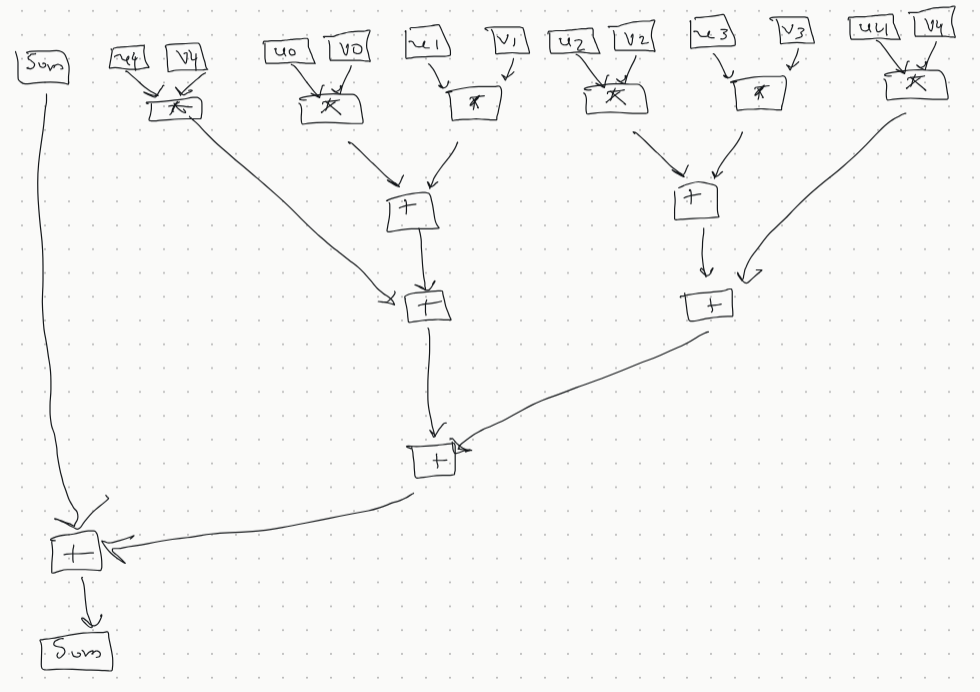
\includegraphics[width=0.7\textwidth]{exercise-05-16}
		\caption{Exercise 5-16: Data dependency flow graph for inner product using
			$6\times 1a$ loop unrolling}
		\label{fig:ex-05-16}
	\end{figure}
\end{sol}

\begin{ex}{5.17}
	The library function \texttt{memset} has the following prototype:
	\begin{lstlisting}
void *memset(void *s, int c, size_t n);
	\end{lstlisting}
	This function fills \texttt{n} bytes of the memory area starting at \texttt{s} with
	copies of the low order byte of \texttt{c}. For example, it can be used to zero out
	a region of memory by giving argument 0 for \texttt{c}, but other values are possible.
	
	\
	The following is a straightforward implementation of \texttt{memset}:
	\begin{lstlisting}
/* Basic implementation of memset */
void *basic_memset(void *s, int c, size_t n)
{
	size_t cnt = 0;
	unsigned char *schar = s;
	while (cnt < n) {
		*schar++ = (unsigned char) c;
		cnt++;
	}
	return s;
}
	\end{lstlisting}
	Implement a more efficient version of the function by using a word of data type
	\texttt{unsigned long} to pack eight copies of \texttt{c}, and then step through
	the region using word-level writes. You might find it helpful to do additional loop
	unrolling as well. On our reference machine, we were able to reduce the CPE from
	1.00 for the straightforward implementation to 0.127. That is, the program is able to
	write 8 bytes every clock cycle.
	
	\
	Here are some additional guidelines. To ensure portability, let $K$ denote the value
	of \texttt{sizeof(unsigned long)} for the machine on which you run your program.
	
	\begin{itemize}
		\item You may not call any library functions.
		\item Your code should work for arbitrary values of \texttt{n}, including when it is
		not a multiple of $K$. You can do this in a manner similar to the way we finish the
		last few iterations with loop unrolling.
		\item You should write your code so that it will compile and run correctly on any
		machine regardless of the value of $K$. Make use of the operation \texttt{sizeof}
		to do this.
		\item On some machines, unaligned writes can be much slower than aligned ones. (On
		some non-x86 machines, they can even cause segmentation faults.) Write your code so
		that it starts with byte-level writes until the destination address is a multiple
		of $K$, then do word-level writes, and then (if necessary) finish with byte-level
		writes.
		\item Beware of the case where \texttt{cnt} is small enough that the upper bounds on
		some of the loops become negative. With expressions involving the \texttt{sizeof}
		operator, the testing may be performed with unsigned arithmetic. (See Section 2.28
		and Problem 2.72.)
	\end{itemize}
\end{ex}

\begin{sol}
	\
	My implementation is below. I included the \texttt{basic\_memset} in the source file
	so I could test my results against it. I used a \texttt{\#define} directive to save
	the length of \texttt{unsigned long} in bytes into a constant \texttt{K}. Then I
	ANDed the address provided by the client with \texttt{K-1} to detect them necessary
	number of iterations to before I would the address aligned on a $K$-byte boundary.
	I replicated the least significant byte of \texttt{c} across a word \texttt{cLSBword}
	via repeated shifting and bit-level OR. Before computing the limit to do word-level writes,
	I was careful to compare \texttt{n - cnt} with \texttt{K} so as to avoid getting a large
	positive number. Then the rest of the method was treated as a $K\times 1$ loop unrolling. 
	\lstinputlisting{17-memset/memset.c}
\end{sol}

\begin{ex}{5.18}
	We considered the task of polynomial evaluation in Practice Problem 5.5 and 5.6, with both
	a direct evaluation and an evaluation by Horner's method. Try to write faster versions of
	the function using the optimization techniques we have explored, including loop unrolling,
	parallel accumulation, and reassociation. You will find many different ways of mixing
	together Horner's scheme and direct evaluation with these optimization techniques.
	
	\
	Ideally, you should be able to reach a CPE close to the throughput limit of your machine.
	Our best version achieves a CPE of 1.07 on our reference machine.
	\[
	a_0 + x(a_1 + x(a_2 + x a_3))
	\]
	\begin{align*}
		a_0+a_1x+a_2x^2+a_3x^3 + a_4x^4 + a_5 x^5\\
		(a_0 + a_1x) + (a_2 + a_3x) x^2 + (a_4 + a_5x)x^4
	\end{align*}
\end{ex}
 

\begin{sol}
	\
	I implemented $10\times 10$ loop unrolling in a procedure I called \texttt{poly\_roll} and
	attained about a factor of 3 improvement over the \texttt{poly} procedure on Practice Problem
	5.5. I tried thinking of how to use Horner's method but I was unable to find a way to eliminate
	the dependency chain with the \texttt{result} variable, which is what limited the
	implementation of \texttt{polyh} on Practice Problem 5.6. I came across someone else's
	implementation where they did factoring and a form of reassociation with which yielded better
	results. I would call this $9\times 3a$, since the unrolling factor is $9$, there are 3
	accumulators, and there is some reassociation. I seemed to get a factor of about $3.8$
	improvement with this version. See the snippet below, also found in
	\texttt{18-polynomial-evaluation/evalpoly.c}:
	\lstinputlisting{18-polynomial-evaluation/evalpoly.c}
\end{sol}
\end{document}
